\documentclass{article}
\usepackage[utf8]{inputenc}
\usepackage{hyperref}
\usepackage{amsmath}
\usepackage{amsfonts}
\usepackage{graphicx}


\title{SPhO Ten Year Series (TYS) with Solutions: 2010 Questions}
\author{
    Solutions available on Victoris\\
    \texttt{victoris.org}
    % new collaborators add your name and contact here!
}

\date{\today}

\begin{document}
\maketitle

\subsection{Question 1}
In 1899, Max Planck introduced the units $\hbar=\frac{h}{2\pi}$, $c$ and $G$, where $h$ is the Planck constant, $c$ is the speed of light in vacuo and $G$ is the Newton gravitational constant so that the force between two bodies of masses $m_1$ and $m_2$ placed a distance $r$ apart is given by 
\[F=G\frac{m_1 m_2}{r_2}\]
(i) In terms of these Planck units, write down the dimensions of mass, length and time. These quantities are called the Planck mass $M_{pl}$, the Planck length $l_{pl}$ and the Planck time $t_{pl}$. [9]\\
(ii) Find the value of $M_{pl}$ in SI (i.e. metres-kilogramme-seconds, mks) units. [2] \\
(iii) Find the ratio
 \[\frac{E_{grav}}{m_e c^2}\] where $E_{grav}$ is the gravitational energy between two electrons separated by a distance equal to the Compton wavelength of an electron of mass $m_e$. [4] \\
(iv) Consider a particle of mass $M_{pl}$. Find the ratio \[\frac{E_{grav}}{M_{pl} c^2}\] where $E_{grav}$  is the gravitational energy between two such particles separated by a distance equal to their own Compton wavelength. Thus, $M_{pl}$ can be interpreted as the mass scale that quantum gravitational effects become important. [2] \\

[Note: The energy of a photon with the Compton wavelength of a particle is the same as the rest mass of the particle.] 

\subsection{Question 2}
2. A block of mass $M$ rests on a fixed plane inclined at angle $\theta$. A horizontal force of $Mg$ is applied to the block, as shown in Fig. \ref{2010q2}. The coefficient of static friction between the block and the plane is $\mu$. \\
(i) Assuming that the friction force between the block and the plane is large enough to keep the block at rest, determine the magnitude of the normal and friction forces (call them $N$ and $F_y$ ) that the plane exerts on the block in terms of $M$ and $\mu$\\
(ii) determine the range of angles $\theta$ for which the block remain at rest on the plane in terms of $\mu$. 

\begin{figure}
\centering
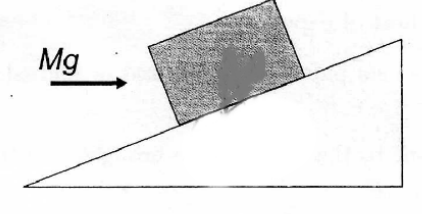
\includegraphics[width=0.5 \linewidth]{spho_book_TYS_images/2010q2.png}
\caption{Horizontal force on a block.} \label{2010q2}
\end{figure}


\subsection{Question 3}
3. A mobile is formed by supporting four metal butterflies of equal mass $m$ from a string of length $L$. The points of support are evenly spaced a distance $\ell$ apart as shown in Figure \ref{2010q3}. The string forms an angle $\theta_{1}$ with the ceiling at each end point. The center section of string is horizontal. \\
(i) Find the tension in each section of string in terms of $\theta_{1}, m$, and $g$. \\
(ii) Find the angle $\theta_{2}$, in terms of $\theta_{1}$. \\
(iii) Show that the distance $D$ between the end points of the string is
$$
D=\frac{L}{5}\left(a \cos \theta_{1}+b \cos \left[\tan ^{-1}\left(\frac{1}{2} \tan \theta_{1}\right)\right]+1\right)
$$
where $a$ and $b$ are constants to be determined. State the values of $a$ and $b$. [3] \\

\begin{figure}
\centering
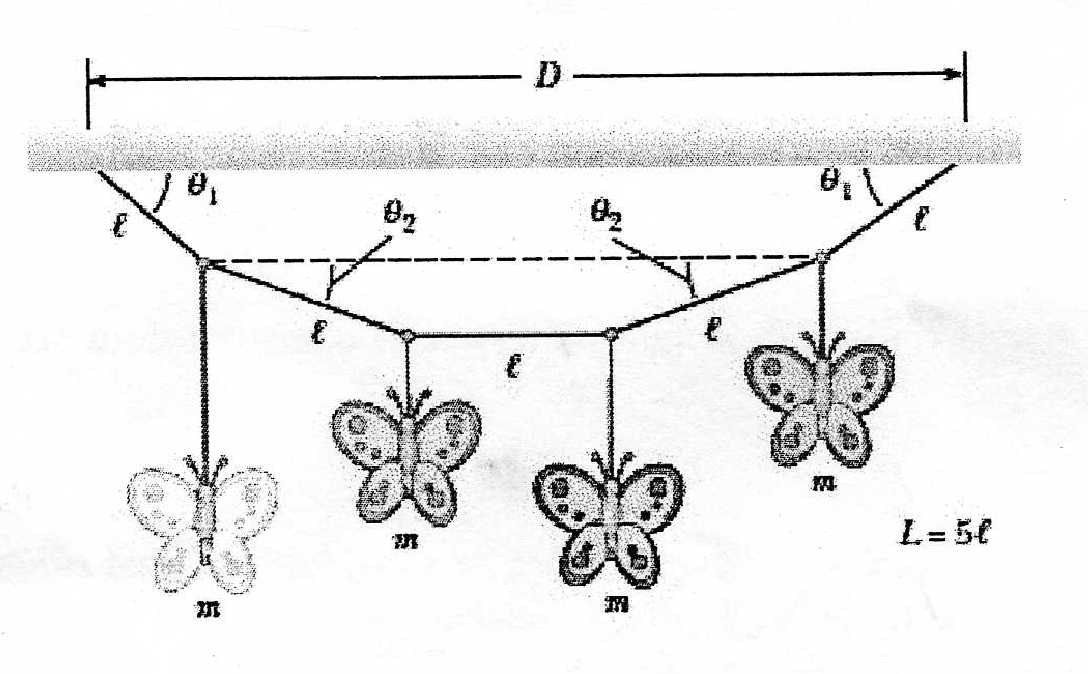
\includegraphics[width=\linewidth]{spho_book_TYS_images/2010q3.png}
\caption{A mobile is formed by supporting four metal butterflies of equal mass $m$.} \label{2010q3}
\end{figure}


\subsection{Question 4}
4. A $670 \mathrm{~kg}$ meteorite is composed of aluminum. At a distance far from the Earth, its temperature is $-15^{\circ} \mathrm{C}$ and it moves with a speed of $14.0 \mathrm{ kms}^{-1}$ relative to the Earth. As it crashes into the planet, the resulting additional internal energy is shared equally between the meteor and the planet. Assuming that all of the material of the meteor rises momentarily to the same final temperature, determine this temperature. You may also assume that the specific heat of liquid and of gaseous aluminum is 1170 $\mathrm{Jkg}^{-1} \mathrm{~K}^{-1}$, the latent heat of fusion and vaporization of aluminum are $3.97 \times 10^{5} \mathrm{~J}$ $\mathrm{kg}^{-1}$ and $1.14 \times 10^{7} \mathrm{~J} \mathrm{~kg}^{-1}$ respectvely, and the melting point and boiling point of aluminum are $660 \mathrm{~K}$ and $2450 \mathrm{~K}$ respectively.
[10]

\subsection{Question 5}
5. A pion at rest with a mass $m_{\pi}$ decays to a muon of mass $m_{\mu}$ and an antineutrino of negligible mass. The reaction is written as $\pi^{-} \rightarrow \mu^{-}+\bar{\nu}$. Calculate the kinetic energy of the muon and the energy of the antineutrino in electron volts. You may take $m_{\pi}=273 m_{e}$ and $m_{\mu}=207 m_{e}$ where $m_{e}$ is the rest mass of the electron.
$[9]$


\subsection{Question 6}
6. A smaller disk of radius $r$ and mass $m$ is attached rigidly to the face of a second larger disk of radius $R$ and mass $M$ as shown in Figure \ref{2010q6}. The center of the small disk is located at the edge of the large disk. The large disk is mounted at its center on a frictionless axle. The assembly is rotated through a small angle $\theta$ from its equilibrium position and released. \\
(i) Show that the speed of the center of the small disk as it passes through the equilibrium position is
$$
v=\alpha\left[\frac{R g(1-\cos \theta)}{(M / m)+(r / R)^{2}+\beta}\right]^{1 / 2}
$$
where $\alpha$ and $\beta$ are constants to be determined. State the values of these constants. [7]\\
(ii) Determine the period of the motion in terms of $M, m, R$ and $r$. [3]
\begin{figure}
	\centering
	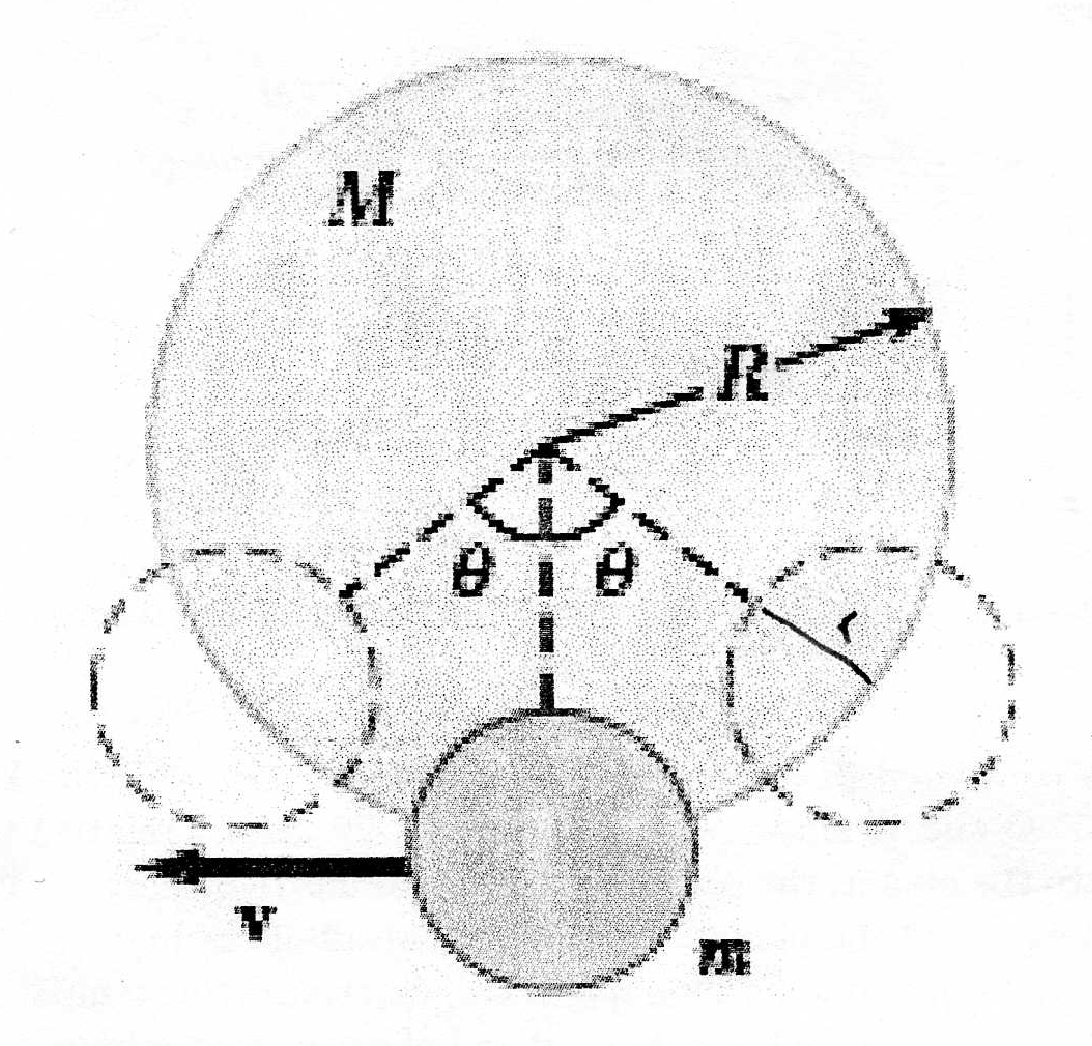
\includegraphics[width=0.5\linewidth]{spho_book_TYS_images/2010q6.png}
	\caption{A smaller disk of radius $r$ and mass $m$ is attached rigidly to the face of a second larger disk of radius $R$ and mass $M$}\label{2010q6}
\end{figure}

\subsection{Question 7}
7. An electric motor turns a flywheel through a drive belt that joins a pulley on the motor and a pulley that is rigidly attached to the flywheel, as shown in Figure \ref{2010q7}. The flywheel is a solid disk with a mass of $80.0 \mathrm{~kg}$ and a diameter of $1.25 \mathrm{~m}$. It turns on a frictionless axle. Its pulley has a much smaller mass and a radius of $0.230 \mathrm{~m}$. If the tension in the upper (taut) segment of the belt is $135 \mathrm{~N}$ and the flywheel has a clockwise angular acceleration of $1.67 \mathrm{rads}^{-2}$, find the tension in the lower (slack) segment of the belt.
$[4]$

\begin{figure}
	\centering
	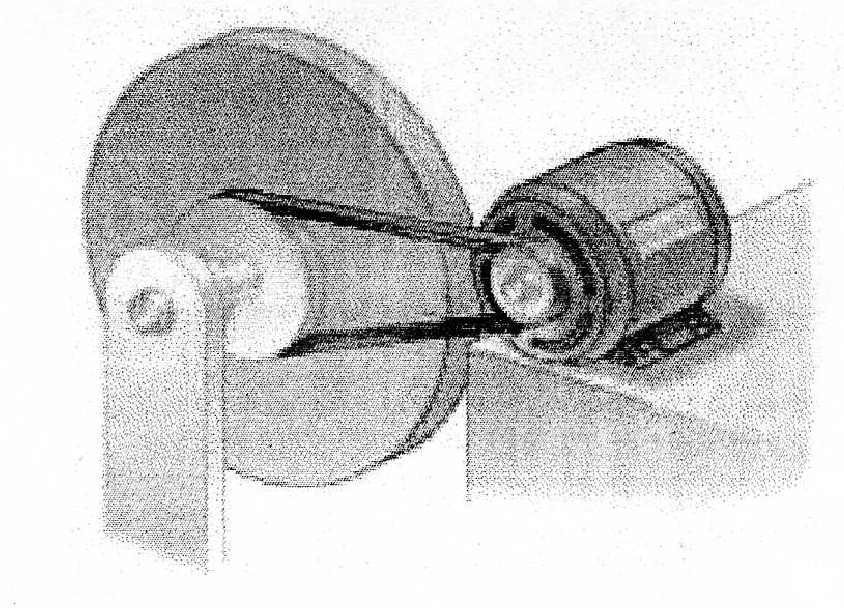
\includegraphics[width=0.5\linewidth]{spho_book_TYS_images/2010q7.png}
	\caption{An electric motor turns a flywheel through a drive belt that joins a pulley on}\label{2010q7}
\end{figure}

\subsection{Question 8}
8. A plano-concave lens having index of refraction $1.50$ is placed on a flat glass plate, as shown in Figure \ref{2010q8}. Its curved surface, with radius of curvature $8.00 \mathrm{~m}$, is on the bottom. The lens is illuminated from above with yellow sodium light of wavelength $589 \mathrm{~nm}$, and a series of concentric bright and dark rings is observed by reflection. The interference pattern has a dark spot at the center, surrounded by 50 dark rings, of which the largest is at the outer edge of the lens. \\
(i) What is the thickness of the air layer at the center of the interference pattern? \\
(ii) Calculate the radius of the outermost dark ring. \\
(iii) Find the focal length of the lens. [9]

\begin{figure}
	\centering
	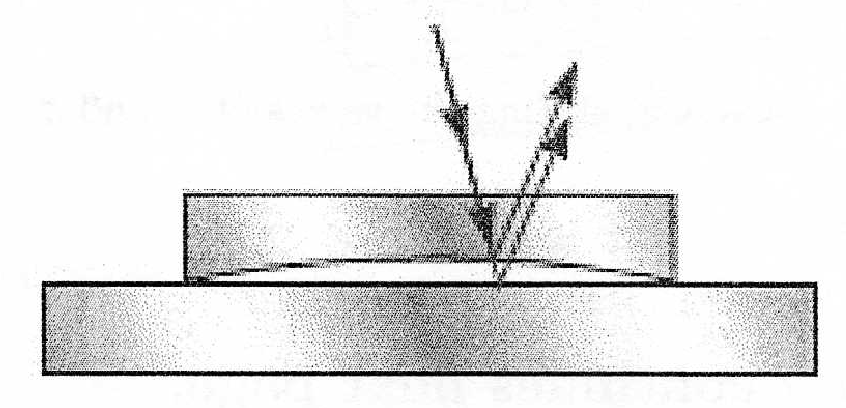
\includegraphics[width=0.5\linewidth]{spho_book_TYS_images/2010q8.png}
	\caption{A plano-concave lens placed on a flat glass plate} \label{2010q8}
\end{figure}

\subsection{Question 9}
9. (a) A toroid has a major radius $R$ and a minor radius $r$ and it is tightly wound with $N$ turns of wire, as shown in Figure \ref{2010q9}. If $R>>r$, the magnetic field in the region enclosed by the wire of the torus, of cross-sectional area $A=\pi r^{2}$, is essentially the same as the magnetic field of a solenoid that has been bent into a large circle of radius $R$.\\
\begin{figure}
	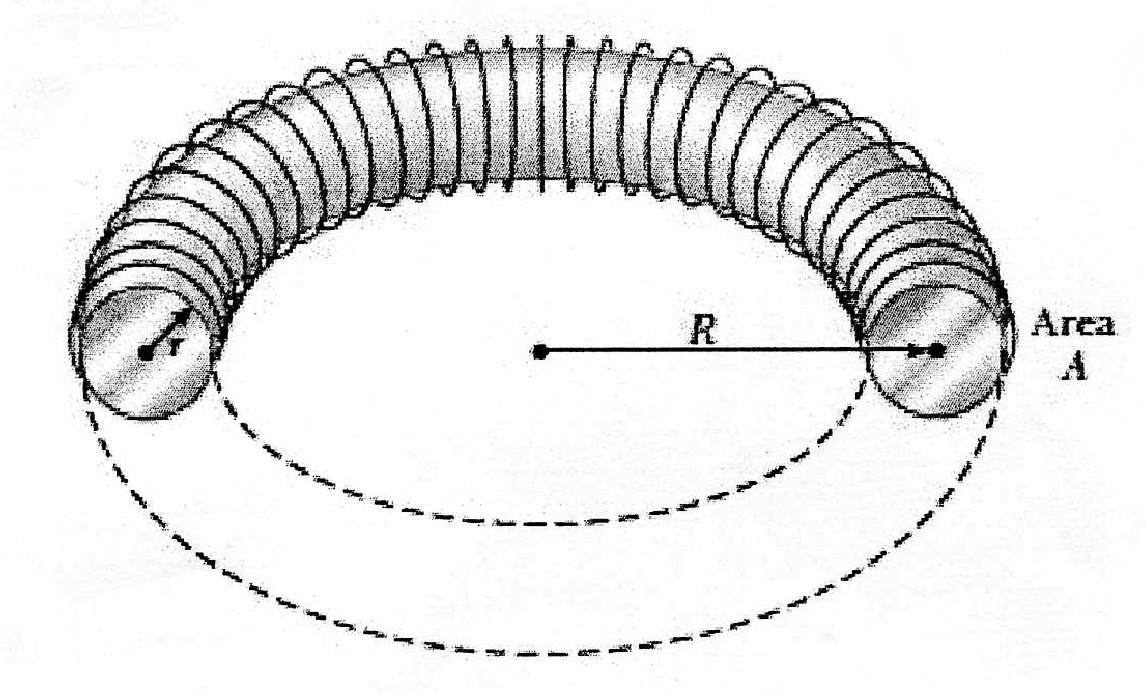
\includegraphics[width=0.8\linewidth]{spho_book_TYS_images/2010q9.png}
	\caption{A toroid has a major radius $R$ and a minor radius $r$ and it is tightly wound with $N$ turns of wire.} \label{2010q9}
\end{figure}
Show that the self-inductance of such a toroid is approximately
$$
L \approx \kappa \mu_{0} \frac{N^{\alpha} A}{R}
$$
where $\kappa$ and $\alpha$ are constants. State the values of $\kappa$ and $\alpha$.
(b) The toroid in Figure \ref{2010q9} with $N$ turns of wire is now replaced by one with a rectangular cross section. Its inner and outer radii are $a$ and $b$, respectively. The cross-section is a rectangle of length $b-a$ and breadth $h$.
(i) Show that the inductance of the toroid is
$$
L=\kappa^{\prime} \mu_{0} \frac{N^{\beta} h}{R} \ln \frac{b}{a}
$$
where $\kappa^{\prime}$ and $\beta$ are constants, stating the values of $\kappa^{\prime}$ and $\beta$ [4]. \\
(ii) Compute the self-inductance of a 500-turn toroid for which $a=10.0 \mathrm{~cm}$, $b=12.0 \mathrm{~cm}$, and $h=1.00 \mathrm{~cm}$. In part (a), an approximate expression for the inductances of a toroid with $R>>r$ was derived. If the calculations in part (b) (ii) were done using this approximate expression for self-inductance, what is the percentage error in the result? \\
\begin{figure}
	\centering
	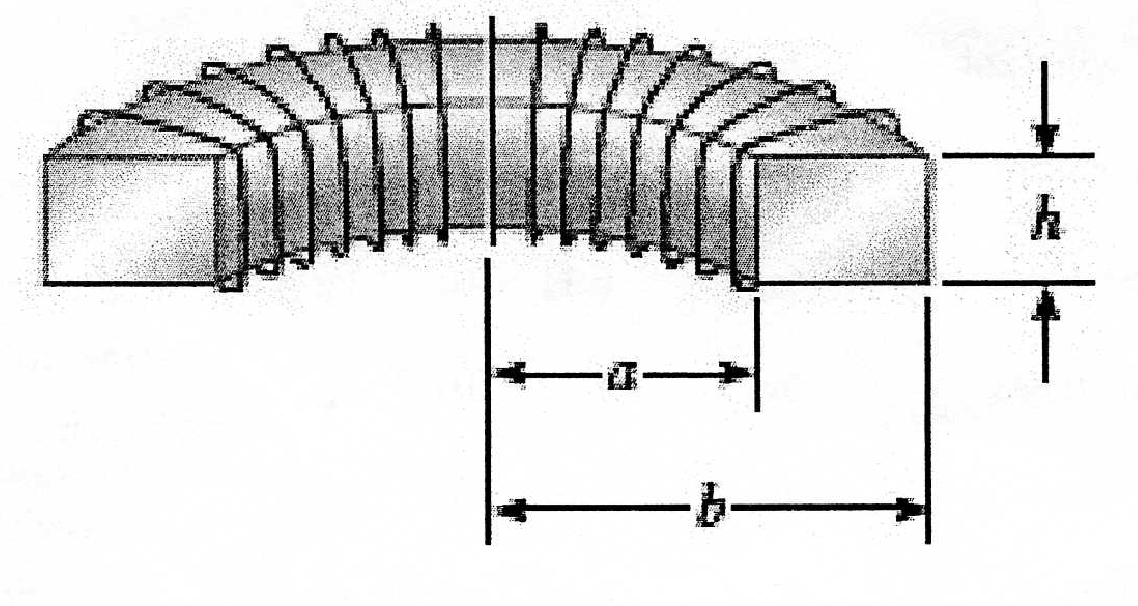
\includegraphics[width=0.8\linewidth]{spho_book_TYS_images/2010q9_2.png}
	\caption{A toroid with a rectangular cross-section.} \label{2010q9_2}
\end{figure}

\subsection{Question 10}
10. An empty box of total mass $M$ with perfectly reflecting walls is at rest in the lab frame. Then electromagnetic standing waves are introduced along the $x$ direction, consisting of $N$ photons, each of frequency $\nu$ as shown in Fig. 8. Determine the rest mass of the system (box + photons) when the photons are present.
\begin{figure}
	\centering
	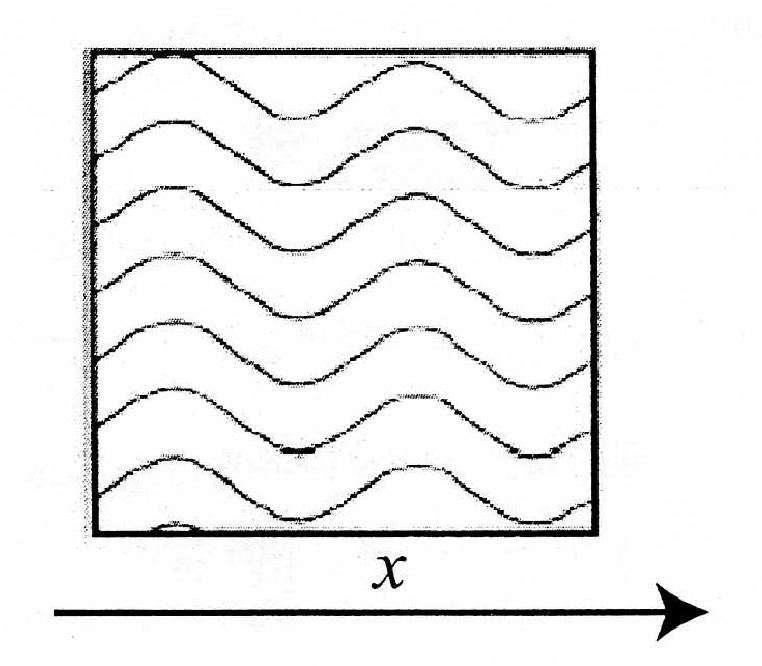
\includegraphics[width=0.5\linewidth]{spho_book_TYS_images/2010q10.png}
	\caption{An empty box of total mass $M$ with perfectly reflecting walls is at rest in the lab frame.}
\end{figure}



\end{document}
